\documentclass{article} % For LaTeX2e
\usepackage{nips13submit_e,times}
% \usepackage[dvips]{graphicx}
% \usepackage[pdftex]{graphicx}
\usepackage{graphicx}
\usepackage{hyperref}
\usepackage{subcaption}
\usepackage{url}
\usepackage{amssymb}
\usepackage{amsmath}
\usepackage{amsthm}
\usepackage{titlesec}
 
\usepackage{float}

\captionsetup{belowskip=-9pt}

\titlespacing*{\section} {0pt}{0pt}{0pt}
\titlespacing*{\subsection} {0pt}{0pt}{0pt}

%\documentstyle[nips13submit_09,times,art10]{article} % For LaTeX 2.09
\title{Deep Learning based Authorship Identification}
\author{
Chen Qian \qquad \qquad \qquad  Tianchang He \qquad  \qquad \qquad  Rao Zhang\\
Department of Electrical Engineering \\
Stanford University, Stanford, CA 94305 \\
\texttt{cqian23@stanford.edu \quad th7@stanford.edu \quad zhangrao@stanford.edu}\\
}
\newcommand{\fix}{\marginpar{FIX}}
\newcommand{\new}{\marginpar{NEW}}
\nipsfinalcopy % Uncomment for camera-ready version
\begin{document}
\maketitle

\begin{abstract}
Authorship identification is an important topic in the field of Natural Language Processing (NLP). It enables us to identify the most likely author of articles, news or messages. Authorship identification can be applied to tasks such as identifying anonymous author, detecting plagiarism or finding ghost writer. In this project, we tackled this problem at different levels, with different deep learning models and on different datasets. Among all models we tested, article-level GRU achieves the best result of 69.1\% accuracy on C50 dataset and 89.2\% on Guternberg dataset. We further studied authorship verification, on which task our Siamese network-based model outputs 99.8\% accuracy on both C50 and Gutenberg.
\end{abstract}
\section{Introduction}
% what is authorship identification
A published author usually has a unique writing style in his works. The writing style is to some extent irrelevant with the topics and can be recognized by human readers. The process of identifying the author from a group of candidates according to his writing samples (sentences,  paragraphs or short articles) is authorship identification.
% the importance of authorship identification
The importance of authorship identification lies on its wide applications. It can be used to find the original author of widely reprinted articles, as well as plagiarised paragraphs. It provides a new way to recommend to a reader the authors who have a high similarity of writing style with his/her favorite authors or anonymous writers, etc.
% the approach we used in our work
In our work, two labelled datasets are adopted to train and test our models. Several most advanced deep learning models are utilized at different levels to evaluate the accuracy of authorship identification.
% the results we obtained in this paper
The contributions of our paper are summarized as follows.
\begin{itemize}
    \item The authorship identification is performed on both a news dataset (Reuters\_50\_50) and a story dataset (Gutenberg) at both sentence level and article level.
    \item Gated Recurrent Unit (GRU) network and Long Short Term Memory (LSTM) network are implemented, tuned and evaluated on the performance of authorship identification.
    \item Siamese network is proposed to examine the similarity of two articles. It proves to be powerful on authorship verification.
\end{itemize}
The rest of this paper is organized as follows. In section 2, we investigate the state-of-the-art of authorship identification models and methods. In section 3, we elaborate the approach of our work, including the datasets and word representations we used, as well as the models we built at sentence and article level. In section 4, the experiments we did and the corresponding results are shown to validate our models. Finally, the conclusions are made in section 6 and the contributions are summarized in section 7.
\section{Related Works}
% related work goes here?
Author identification is by far the most prevalent field of authorship analysis in terms of published studies \cite{pan2014}. In \cite{best_known}, the authors proposed an the unmasking method, which seems to be the best known method in this field. Support vector machine (SVM) classifier is introduced to attribute questioned documents to authors. In this method, long documents can be effectively distinguished, however, it is not ideal for short ones \cite{shortcoming}. Authorship identification studies advance rapidly in recent years, with the development of scientific research such as information retrieval and deep learning, as well as the well-organized text data sets on the Internet. More recently, an effective method was introduced in \cite{Koppel} which transforms authorship veriifcation to authorship identification using documents found in external sources \cite{pan2014}. The most recent studies of authorship identification are primarily based on machine learning approaches, such as deep neuron networks and succeed with the application of various vector representations of words \cite{Rhodes}.



\section{Approach}
In this section, the approaches of authorship identification we took are elaborated in the following order: datasets, data pre-processing and models.
\subsection{datasets}
In our work, two different datasets are exploited to train and test our model. The two datasets are Reuters\_50\_50 news dataset and Gutenberg story dataset respectively. The Reuters\_50\_50 dataset is a widely used dataset for authorship identification and the Gutenberg is a dataset established by ourselves.
\subsubsection{Reuters\_50\_50}
The Reuters\_50\_50 (C50) dataset is a subset of RCV1. RCV1 (Reuters Corpus Volume I) an archive of over 800,000 manually categorized newswire stories recently made available by Reuters, Ltd. for research purposes. \cite{RCV} These corpus has already been used in author identification experiments. In the top 50 authors (with respect to total size of articles) were selected. 50 authors of texts labeled with at least one subtopic of the class CCAT (corporate/industrial) were selected. That way, it is attempted to minimize the topic factor in distinguishing among the texts. The training corpus consists of 2,500 texts (50 per author) and the test corpus includes other 2,500 texts (50 per author) non-overlapping with the training texts.\cite{Reuter} In our work, we re-organize these 5000 texts into non-overlapping 9:1 ratio as train set to test set.
\subsubsection{Gutenberg}
The Gutenberg dataset is a story dataset collected and labeled by ourselves. Project Gutenberg \cite{Gutenberg}  offers over 53,000 free e-books on the Internet. On this website, we collected multiple stories of 50 authors among the top 100 most popular authors and built up the dataset. The stories cover a wide variety of topics and styles in order to minimize the topic factor as well. During the process of collecting, we manually reduced some noise contained in the text, such as page number table of contents and information of the contributors. For each author, we selected 900 paragraphs from his/her stories, hence 45000 paragraphs are maintained in our corpus. We split them into non-overlapping 9:1 ratio as train set to test set.

\subsection{Data Pre-Processing}
The pre-processing of the data in our work primarily consists of two parts. They are respectively word representations and input batch alignment.


%
\subsubsection{Word Representations}
In this project, we used the GloVe \cite{glove} word vectors of size 50 as the pretrained word embeddings. The vocabulary contains 400,000 tokens. The GloVe vectors were used to initialize the word embeddings and the gradient are propagated to the embeddings.

Since we used glove.6B.50 as a look-up table to represent our words, there could exist rarely-seen words which cannot be represented.
Hence, we eliminated the occurrences of numbers and special characters to match the feature of our word representations. During the process of parsing, we trimmed each word to ensure that it does not contain any number or special character at both of its ends.

\subsubsection{Input Batch Alignment}
% why do we use batch input?
In our experiment, batch input is adopted to make use of the parallel computing advantage of graphical processing unit (GPU), in order to accelerate the training process of our model. 
% why do we has a fixed input size?
Since the batch has a fixed length as input, we truncated the input if it exceeds the fixed length. If the input doesn't reach the fixed length, we append several "magic word" to the end of the input. The "magic word" is a word created by ourselves, which doesn't exist in the world.
% why do we introduce magic word and masks?
In addition, words which cannot be found in the GloVe look-up table are also replaced by the "magic word". To eliminate the impact of the "magic words" on the result, we masks these words at the output, making the back-propagation of errors ignore these "magic words" and only extract the "real words" from the network.

\subsection{Models}

In this section, we elaborate the deep learning models we used in our experiment. In total four models are implemented: sentence-level GRU, article-level GRU, article-level LSTM, article-level Siamese network.

\subsubsection{Sentence-Level GRU}
Sentence-level GRU predicts author on a small number (typically 3) of continuous sentences, which we call a sentence bundle cropped from an article. 
%
\begin{align}
\label{eq: gru}
\begin{cases}
z_t&=  \sigma(W^{(z)}x_t + U^{(z)}h_{t - 1} + b^{(z)})\\
r_t&= \sigma(W^{(r)}x_t + U^{(r)}h_{t - 1} + b^{(r)}) \\
\tilde{h_t} &= \tanh(r_t \circ U^{(h)}h_{t-1} + W^{(h)} x_t + b^{(h)}) \\
h_t &= (1 - z_t) \circ \tilde{h_t} + z_t \circ h_{t - 1}
\end{cases}  
\end{align}
%
In this model, the input unit is a word. For each time stamp, one word, represented as a word vector is sent to the GRU network,  updating the hidden state and producing some output. The equation for hidden state update and output computation is given in Eq. \ref{eq: gru}. Notice that $h_t$ represents both the new hidden state and the output. After the last word in the sentence bundle is processed, all outputs at previous time stamp are sent to a pooling layer, whose output is simply the average of all inputs. Finally, the output of pooling layer will be used as the input of a softmax classifier, where loss will be calculated and the final decision that which author wins out will be determined. One thing to highlight is that the gradients must be propagated to the embedding layer. The model is shown in Figure \ref{fig: gru_sentence}.
%
\begin{figure}[H]
\centering
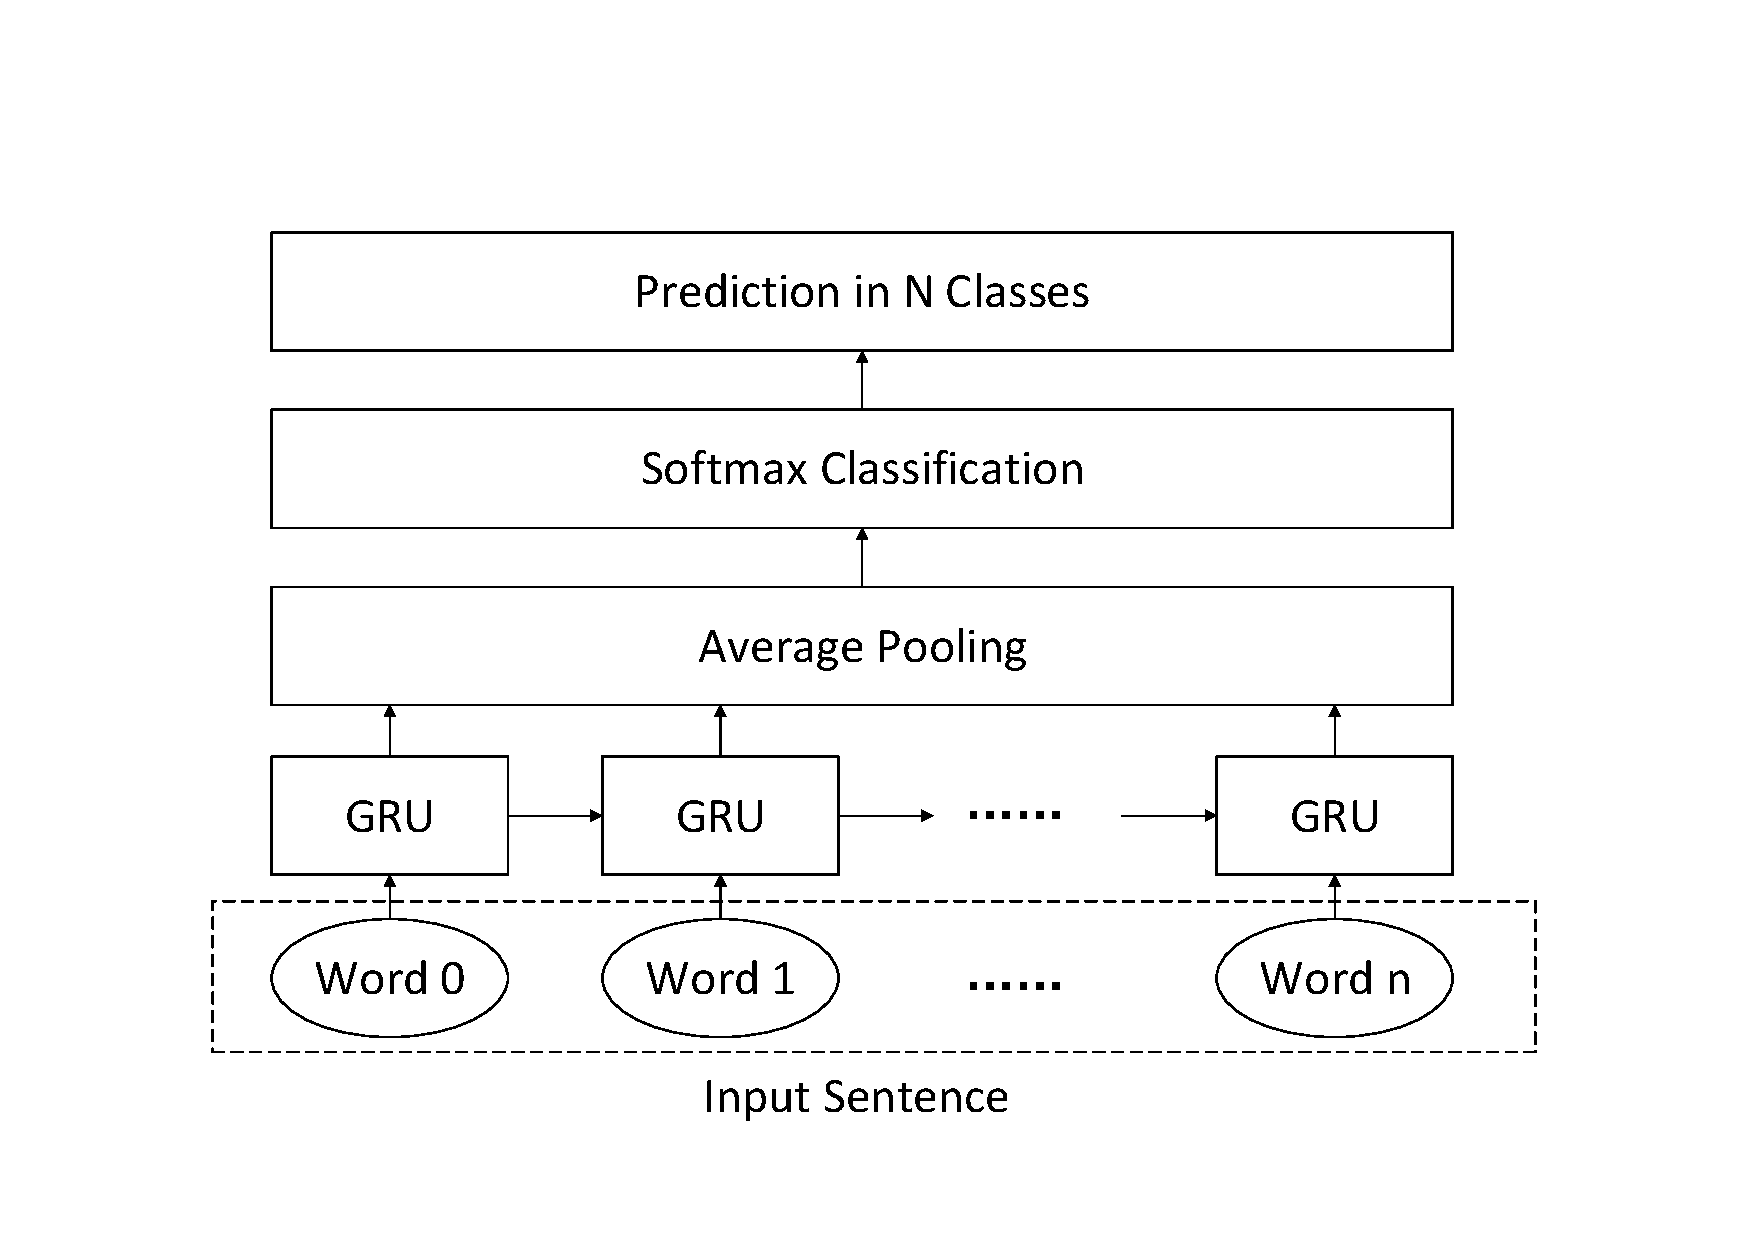
\includegraphics[width = 56mm, height = 40mm]{figures/sentenceLevelGru.pdf} 
\caption{Sentence Level GRU Diagram}
\label{fig: gru_sentence}
\end{figure}
%
The idea beneath this model is to capture an article's style at sentence level. Although it seems impractical to infer an author's style from several sentences, this model in fact has reasonable performance in numerical test, which will be discussed in Section 4. 

\subsubsection{Article-Level GRU}
Different from sentence-level GRU, article-level GRU takes a whole or more paragraphs as the input, and predict its author. In this model, the input unit is a sentence. For each time stamp, a complete sentence represented by the average of all its words' vectors is sent to the model.  Same as the sentence-level model, hidden state will be updated and an output will be produced upon each input using Eq. \ref{eq: gru}. All of the outputs will be sent to an average pooling layer when no more input appears, whose output is the average of its input. Finally, a softmax classifier works on the output of average pooling layer to make the decision which author wins out. The model structure is shown in Figure \ref{fig: gru_article} .

\begin{figure}[htbp]
\centering
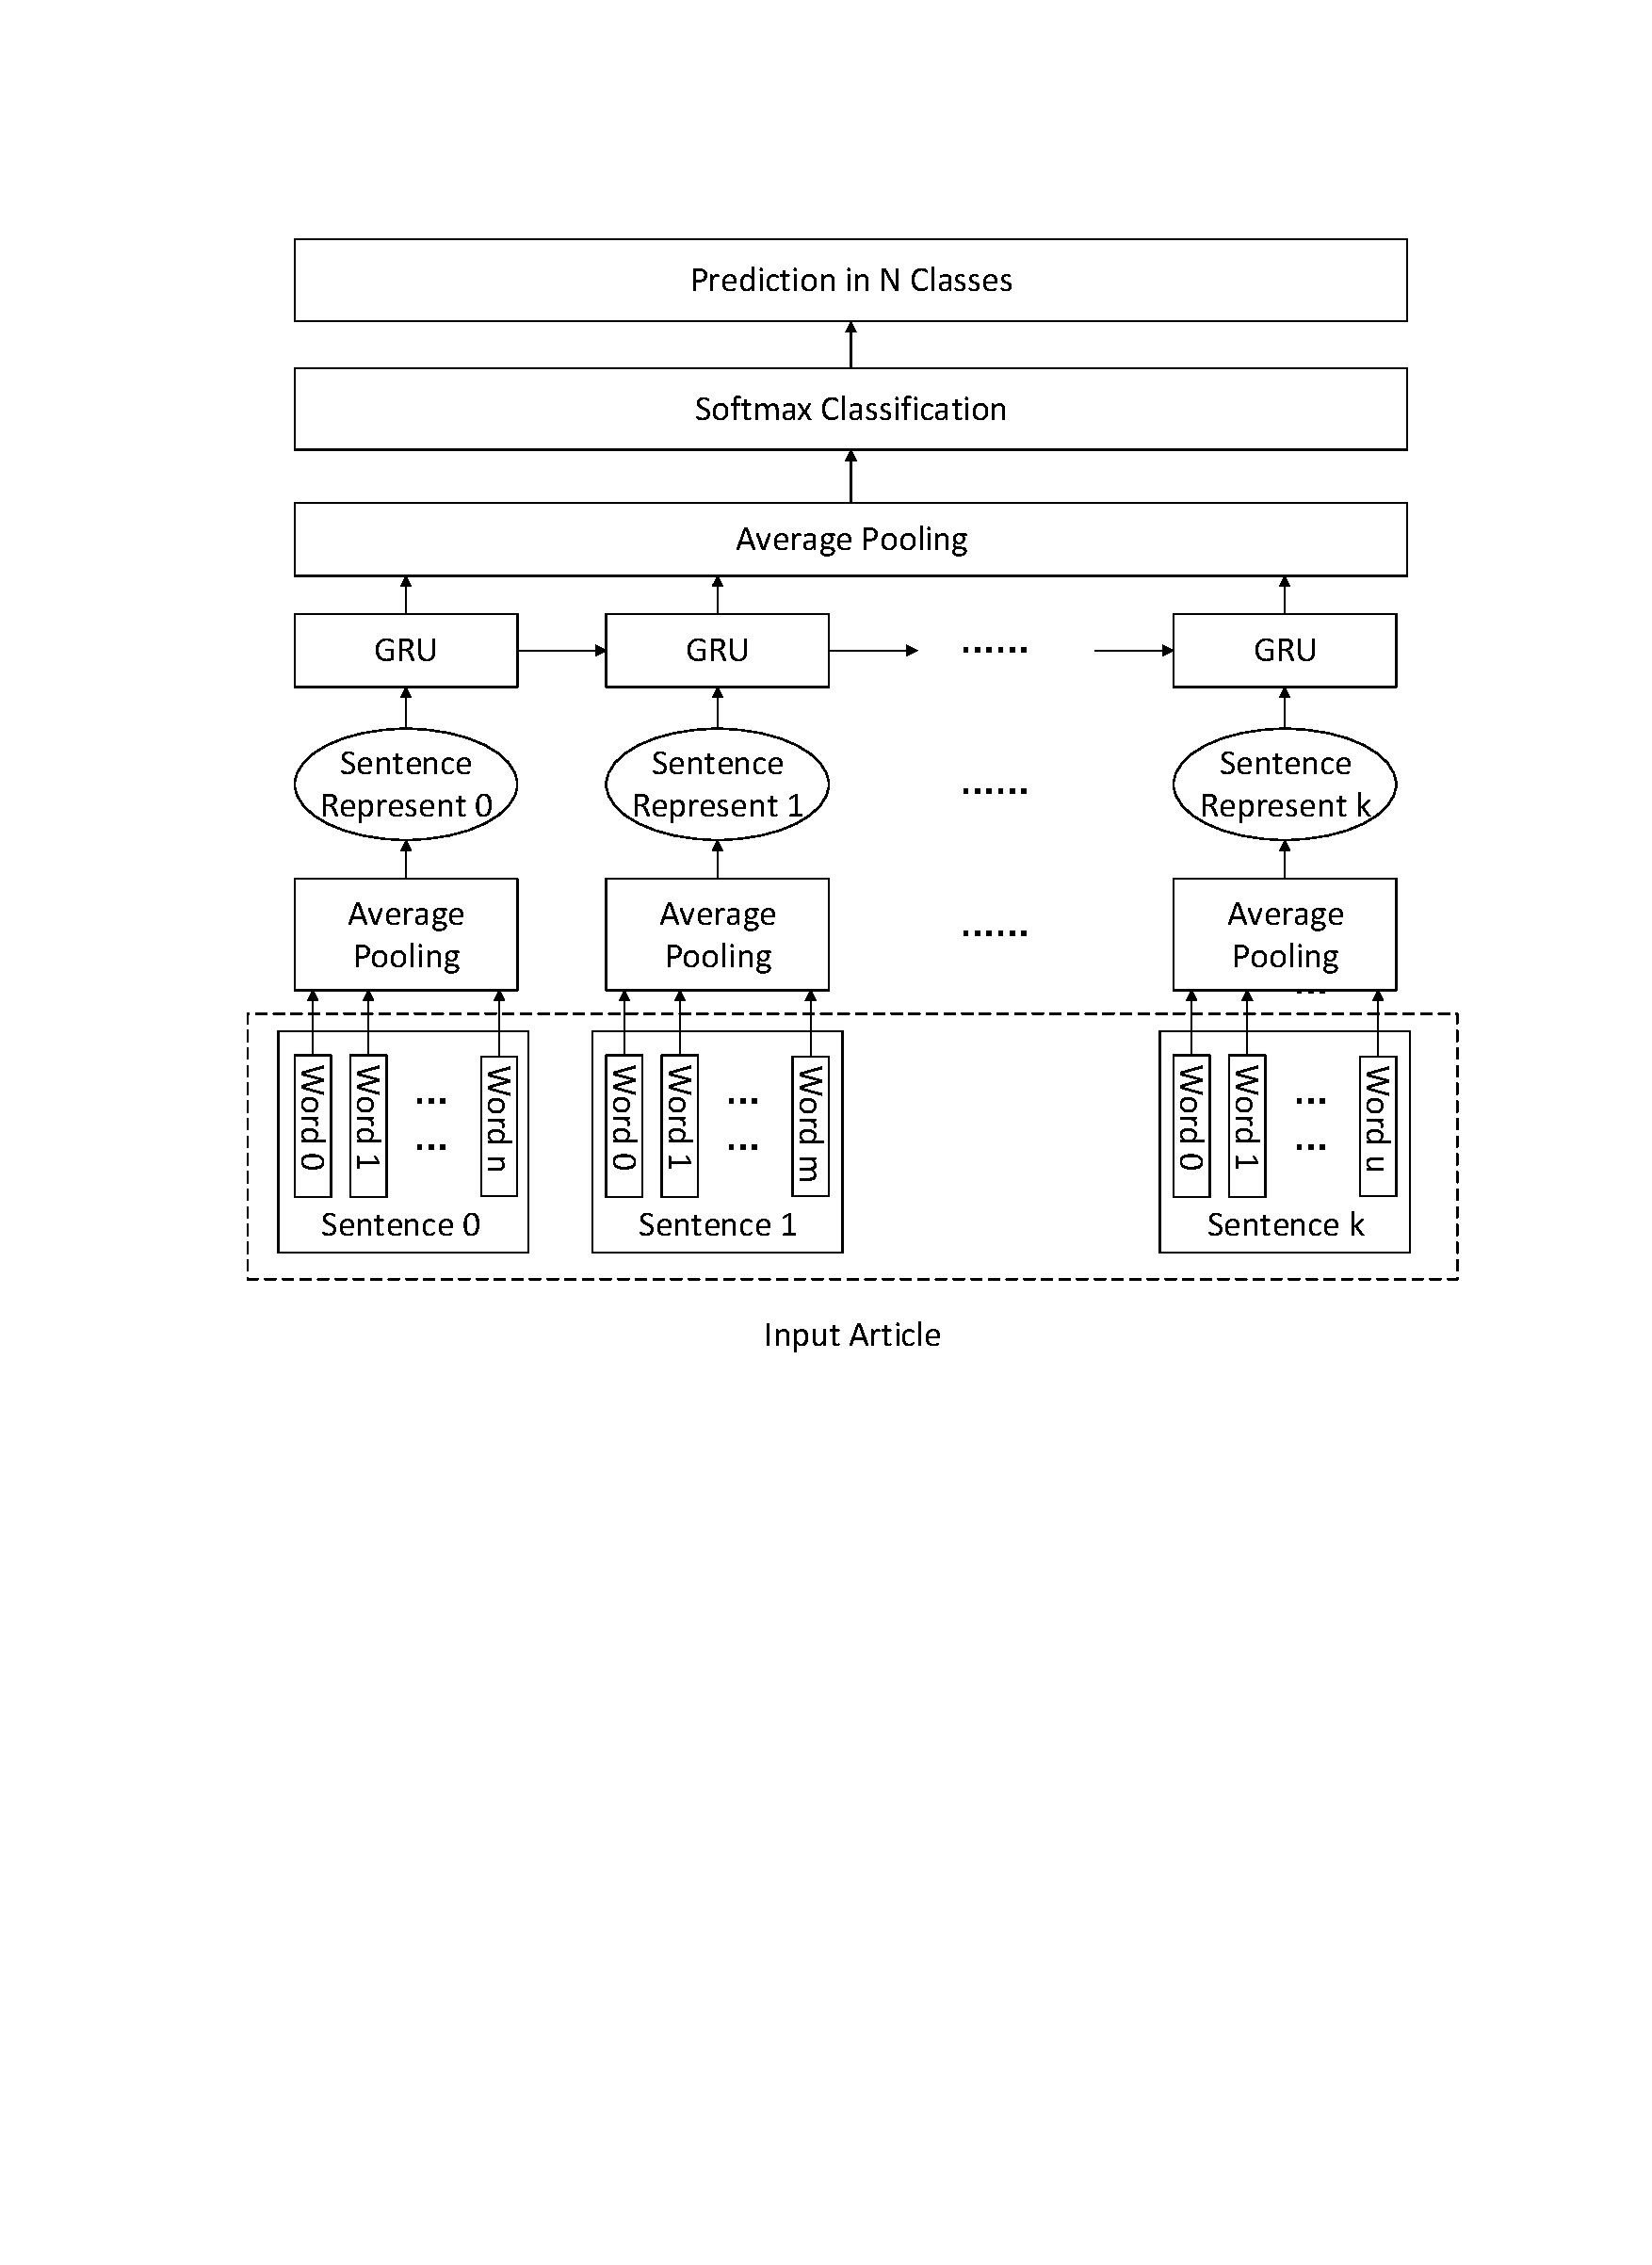
\includegraphics[width = 60mm, height = 50mm]{figures/articleLevelGru.pdf} 
\caption{Article Level GRU Diagram}
\label{fig: gru_article}
\end{figure}


\subsubsection{Article-Level LSTM}

Article-level LSTM is quite similar to the article-level GRU, sharing the same type of input and data representation, and even the structure of the model, as shown in Figure \ref{fig: aLSTM}. The only difference lies on the cell: in LSTM model, we use Eq. \ref{eq: lstm} instead of Eq. \ref{eq: gru}. 
\begin{align}
\label{eq: lstm}
\begin{cases}
i_t&=  \sigma(W^{(i)}x_t + U^{(i)}h_{t - 1} + b^{(i)})\\
f_t&= \sigma(W^{(f)}x_t + U^{(f)}h_{t - 1} + b^{(f)}) \\
o_t&= \sigma(W^{(o)}x_t + U^{(o)}h_{t - 1} + b^{(o)}) \\
\tilde{c_t} &= \tanh(W^{(c)}x_t + U^{(c)} h_{t - 1} + b^{(c)}) \\
c_t&= f_t \circ c_{t - 1} + i_t \circ \tilde{c_t} \\
h_t &= o_t \circ \tanh(c_t)
\end{cases}  
\end{align}
%
\begin{figure}[H]
\centering
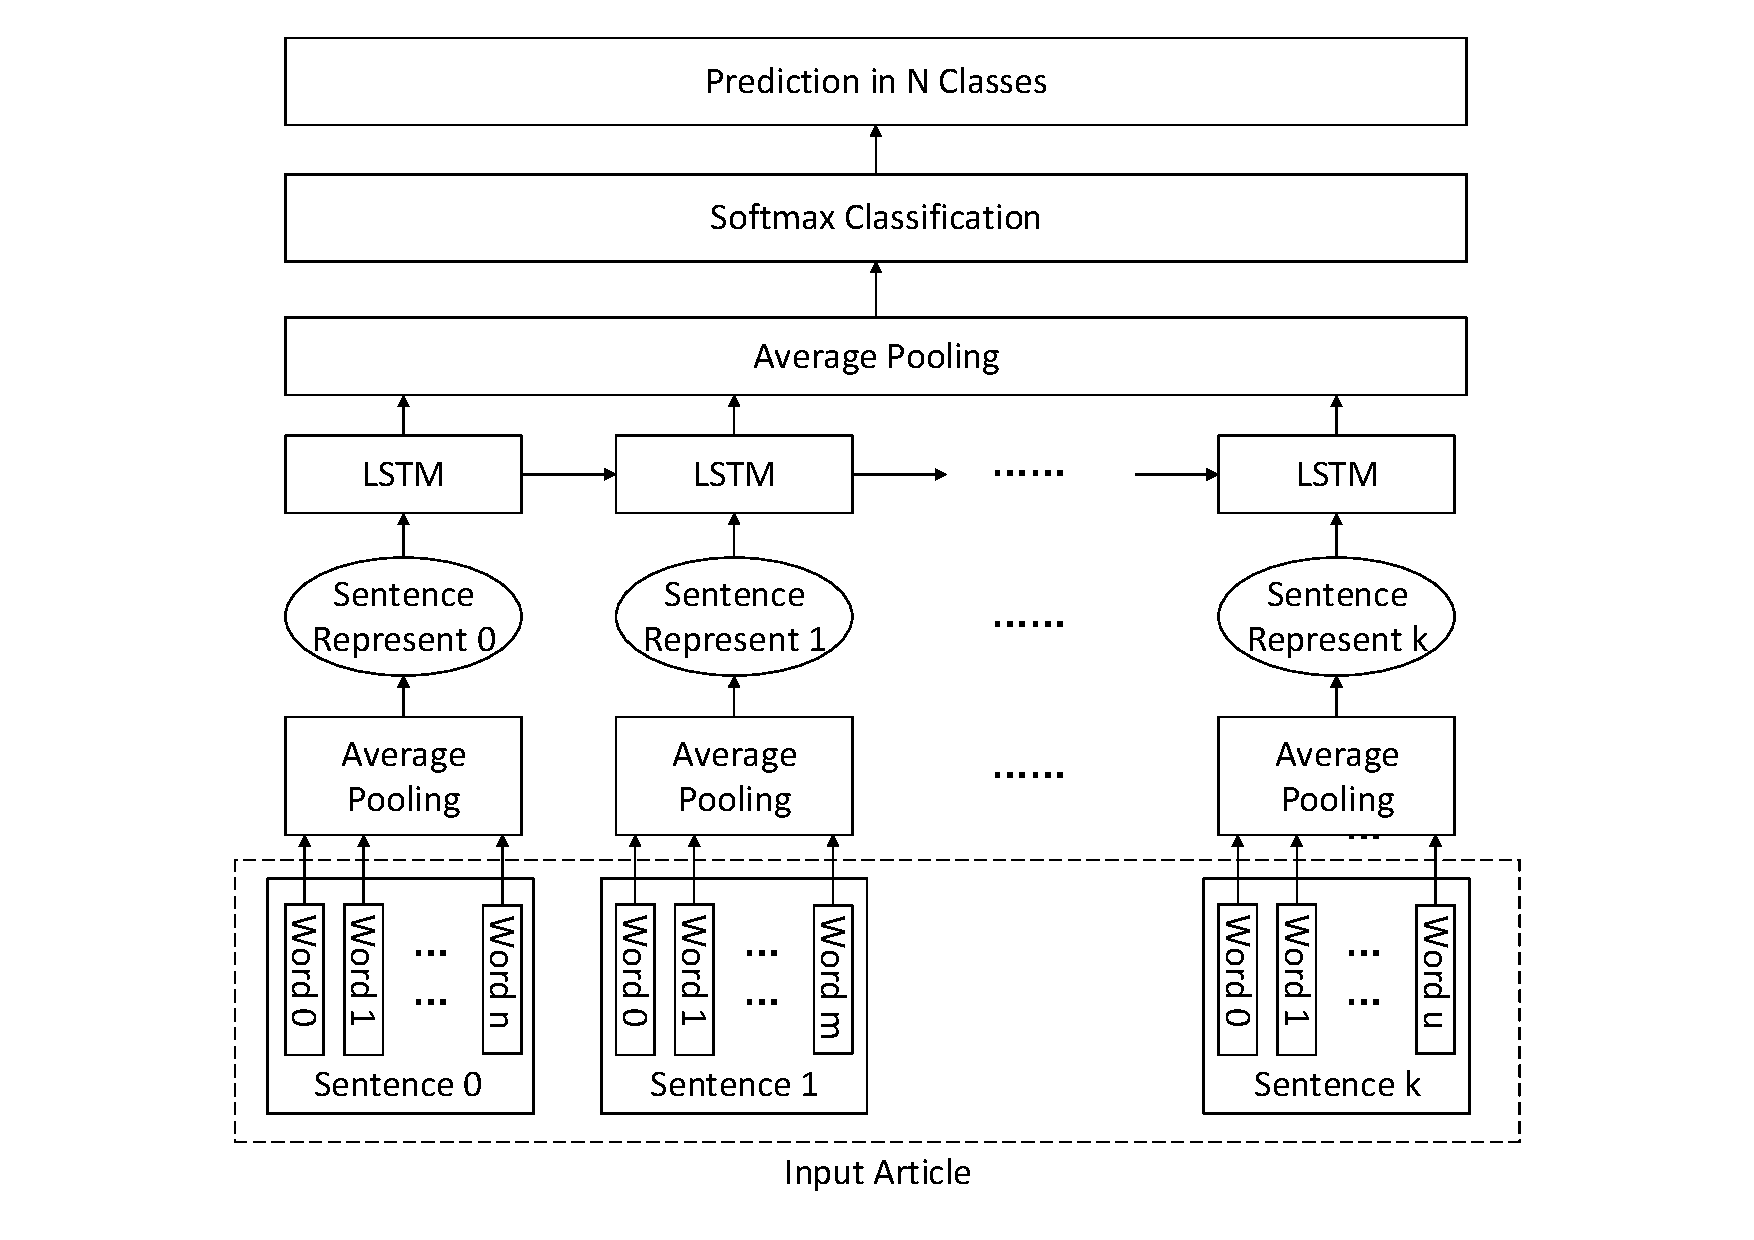
\includegraphics[width=65mm, height = 50mm]{figures/articleLevelLSTM.pdf} 
\caption{Article Level LSTM Diagram}
\label{fig: aLSTM}
\end{figure}
%

\subsubsection{Article-Level Siamese Network}

Siamese network proves to be powerful on verification task, that is, determining whether two input are of the same label. Although we mainly focus on authorship attribution, which is a typical identification job, it is meaningful to look into the verification job, where we make assertion whether two given articles are written by the same author. 

\begin{figure}[H]
\centering
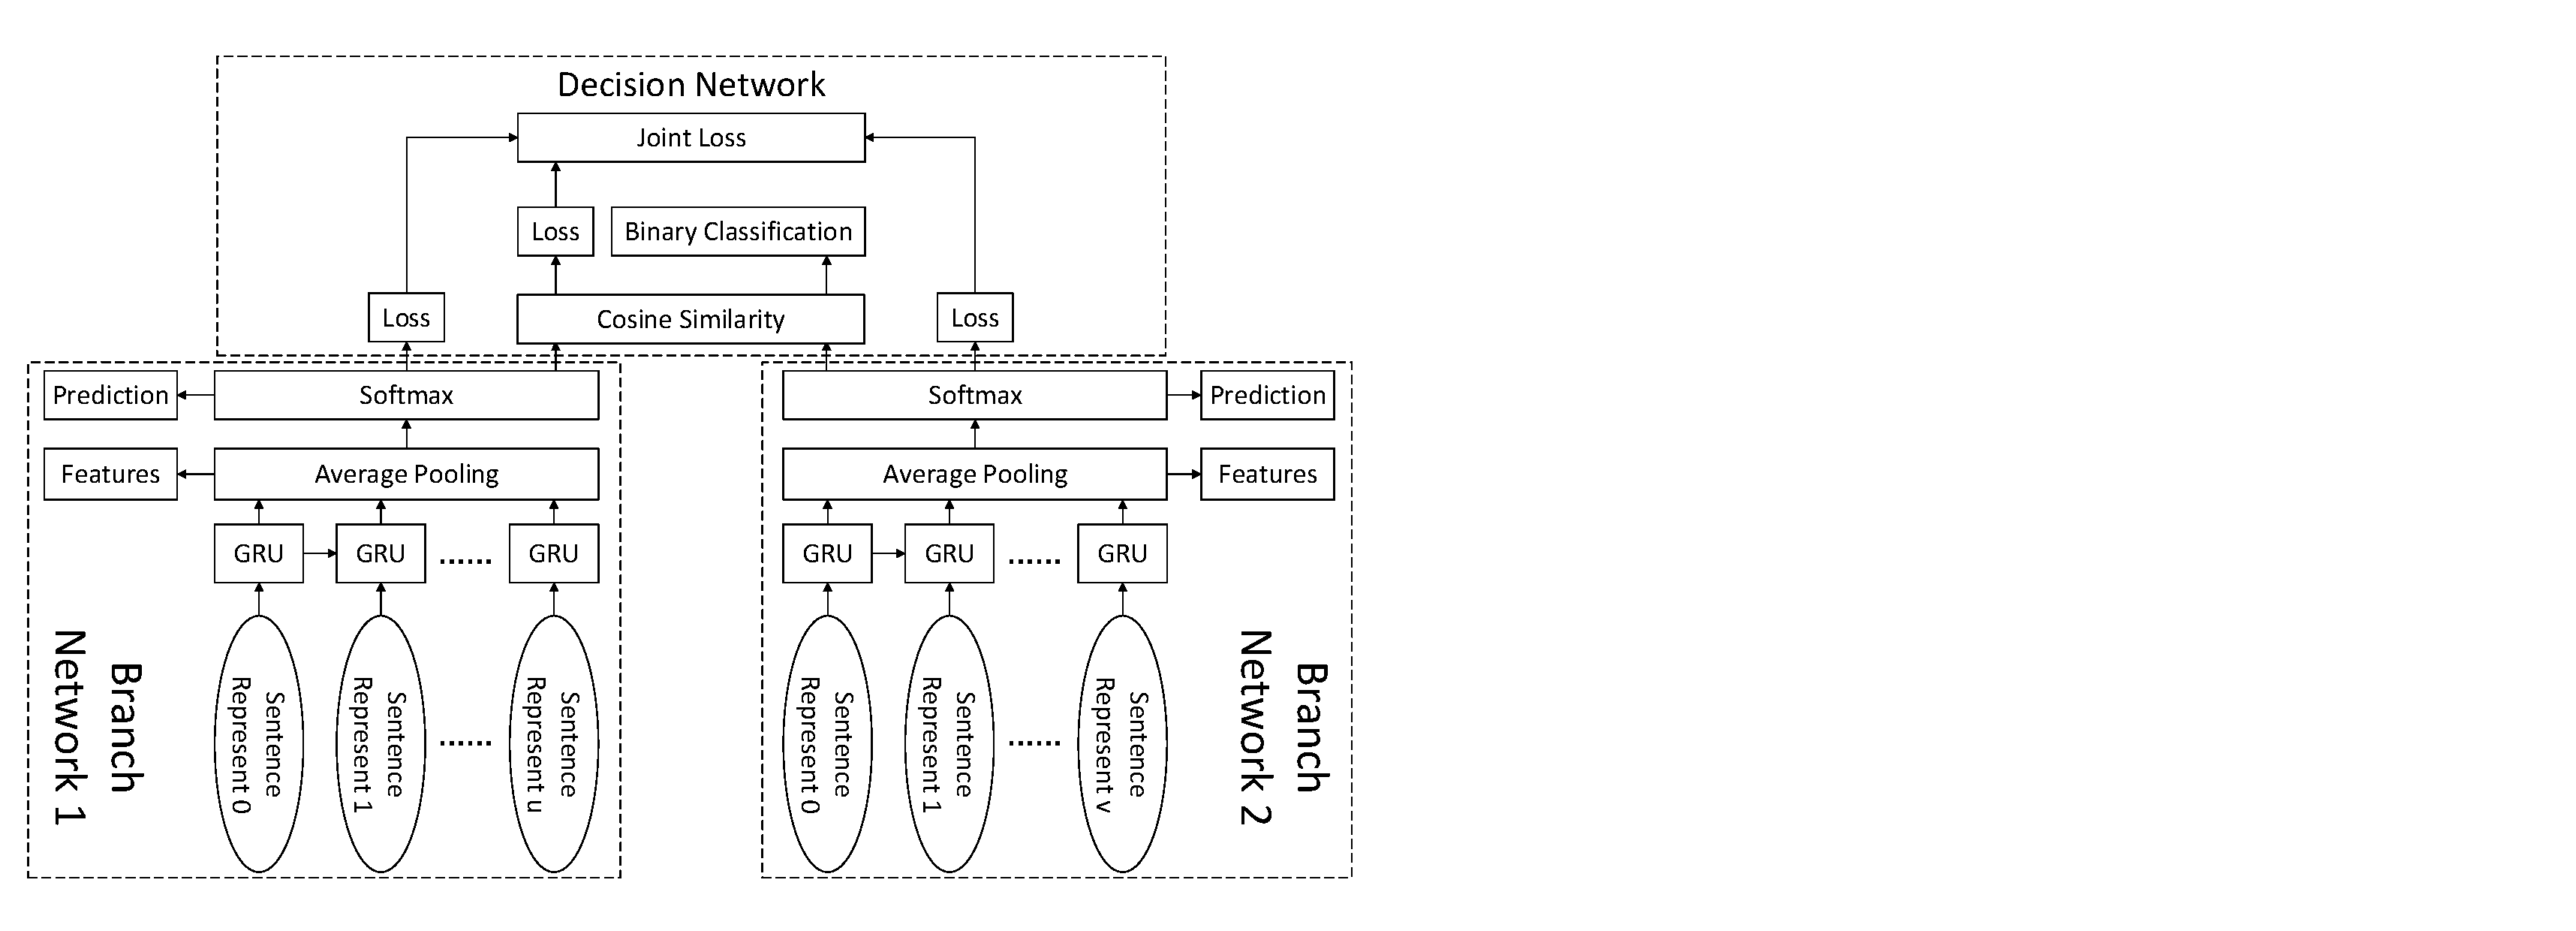
\includegraphics[width=100mm, height = 60mm]{figures/siameseNetwork.pdf} 
\caption{Siamese Network Diagram}
\label{fig: siamese}
\end{figure}

The structure Siamese network, shown in Figure \ref{fig: siamese} largely depends on our article-level GRU model. In specific, two GRU networks sharing all parameters will work separately for two input. The output of the average layer is treated as the extracted features from the input, which will be sent to a similarity measure layer to compute the similarity. As proved in previous work, cosine similarity works better than some other metrics such as Euclidean distance. Thus, cosine similarity is applied in the similarity measure layer. Furthermore, joint loss function is exploited in this model, as shown in Eq. \ref{eq: joint}.
%
\begin{equation}
\label{eq: joint}
J = -\sum\limits_{i = 1}^{n} y_i \log(\hat{y}_i)  -\sum\limits_{j = 1}^{n} y_j \log(\hat{y}_j) + \lambda \sigma(w d(f_1, f_2) + b),
\end{equation}
%
where $d(f_1, f_2)$ is the cosine similarity between $f_1$ and $f_2$:
\begin{equation}
d(f_1, f_2) = \frac{f_1 \cdot f_2}{||f_1||_2 \cdot ||f_2||_2 }
\end{equation}
%
The first two items in Eq. \ref{eq: joint} refer to the identification loss, which comes from classification task, and the third item is referred as verification loss, which comes from verification task. 


This model proves to be extremely powerful in experiment, which we will cover in the next section. 


\section{Experiment \& Result}



\subsection{Baseline}
On the RCV C50 dataset, a baseline accuracy of 12.24\% was achieved \cite{garbage} using Gradient Boosting Classifier with 3 high-level features including Average Word Length, Average Sentence Length, Hapax Legomenon Ratio (fraction of unique words).
%
\subsection{Sentence-Level GRU}
We tested out model using the C50 dataset. We varied the hidden size of GRU network from 50 to 300. The results are shown in \ref{fig: word_c50}. It shows that the larger the hidden size, the higher the accuracy. However, this model is problematic in: 1. The test accuracy is too low compared to training accuracy. 2. The test accuracy is increasing as training accuracy increases. We concluded that this model has too few input and too many parameters and it could lead to overfitting on the training set. We then moved on to operate on the level of articles where we are feeding in a sentence into RNN cell at each time step. 


\begin{figure}[H]
\begin{subfigure}{0.5\linewidth}
\centering
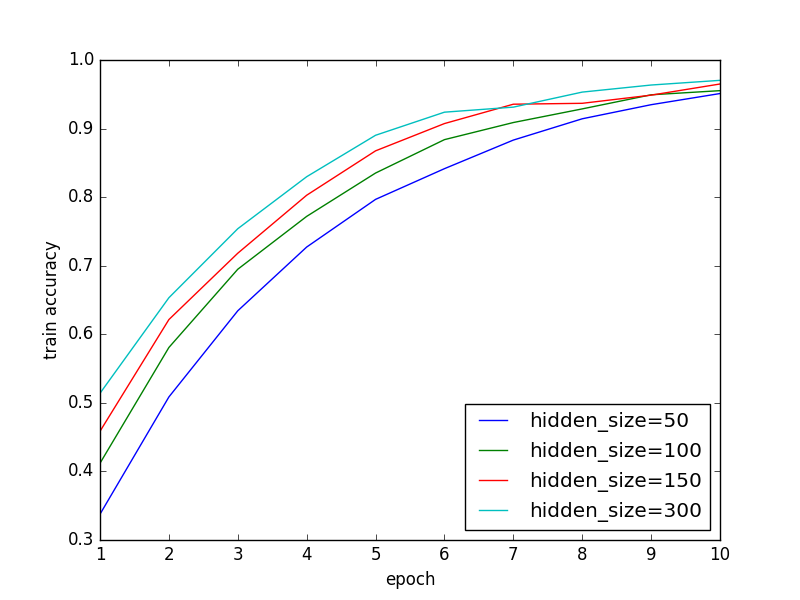
\includegraphics[width=0.7\textwidth]{figures/epoch_train_accu_word_c50.png} 
\caption{Train accuracy cs epoch. }
\end{subfigure}
\begin{subfigure}{0.5\linewidth}
\centering
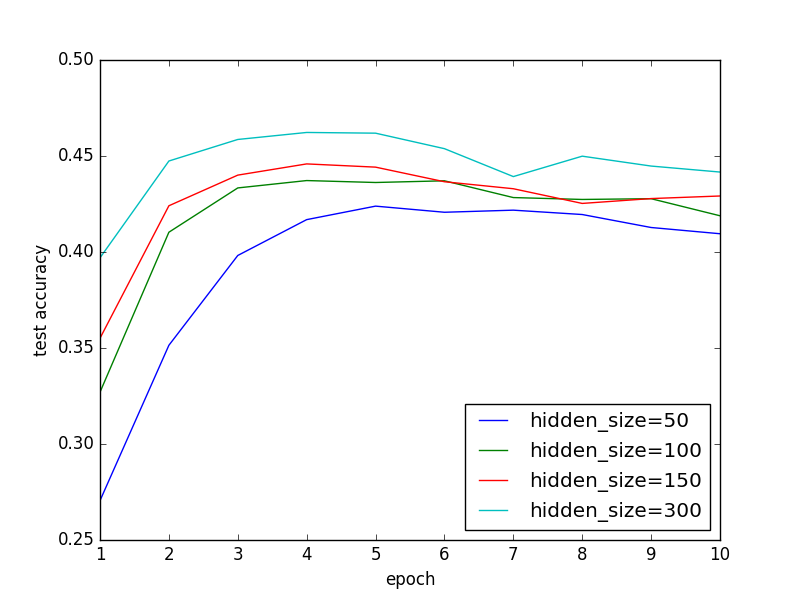
\includegraphics[width=0.7\textwidth]{figures/epoch_test_accu_word_c50.png} 
\caption{Test accuracy vs epoch.}
\end{subfigure}
\caption{Train and test accuracy for different hidden size on C50 dataset.}
\label{fig: word_c50}
\end{figure}


\subsection{Article-Level GRU}
For this model, we did extensive testing. We tested out model using both the C50 dataset and the Gutenberg dataset. We first varied the hidden size of GRU network. The results are shown in Figure \ref{hs_test_accu_c50_ag} and Figure \ref{hs_test_accu_gutenberg_ag}.
%
\begin{figure}[H]
\begin{subfigure}{0.5\linewidth}
\centering
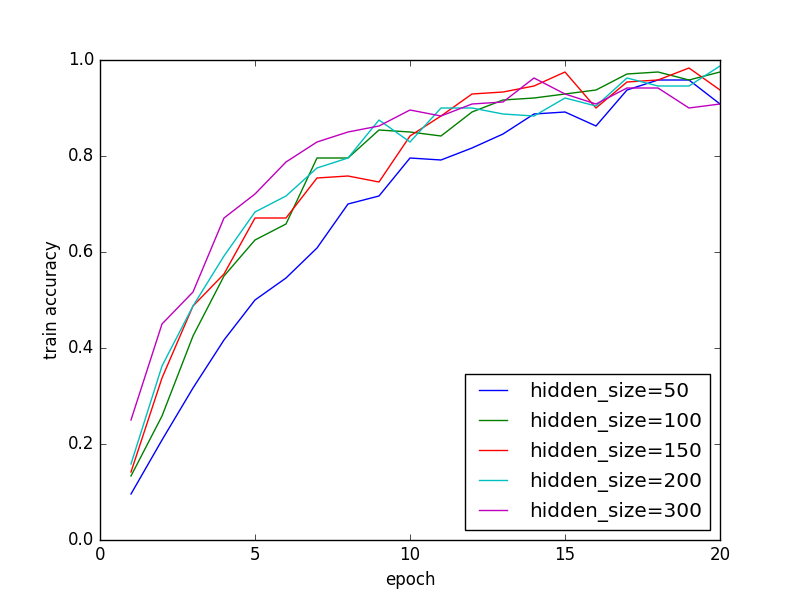
\includegraphics[width=0.7\textwidth]{figures/epoch_train_accu_hs_c.png} 
\caption{Training accuracy vs epoch.}
\end{subfigure}
\begin{subfigure}{0.5\linewidth}
\centering
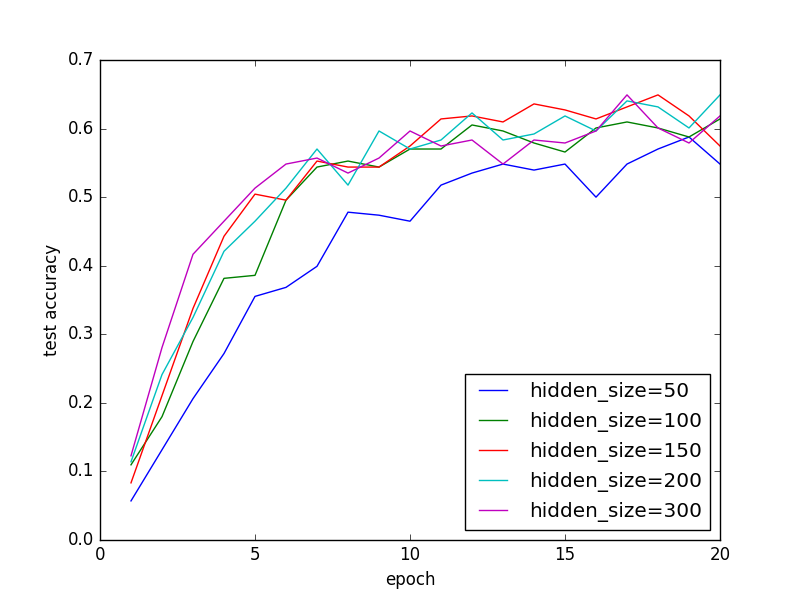
\includegraphics[width=0.7\textwidth]{figures/epoch_test_accu_hs_c.png} 
\caption{Testing accuracy vs epoch.}
\end{subfigure}
\caption{Training and test accuracy for different hidden size on the C50 dataset.}
\label{hs_test_accu_c50_ag}
\end{figure}
%
\begin{figure}[H]
\begin{subfigure}{0.5\linewidth}
\centering
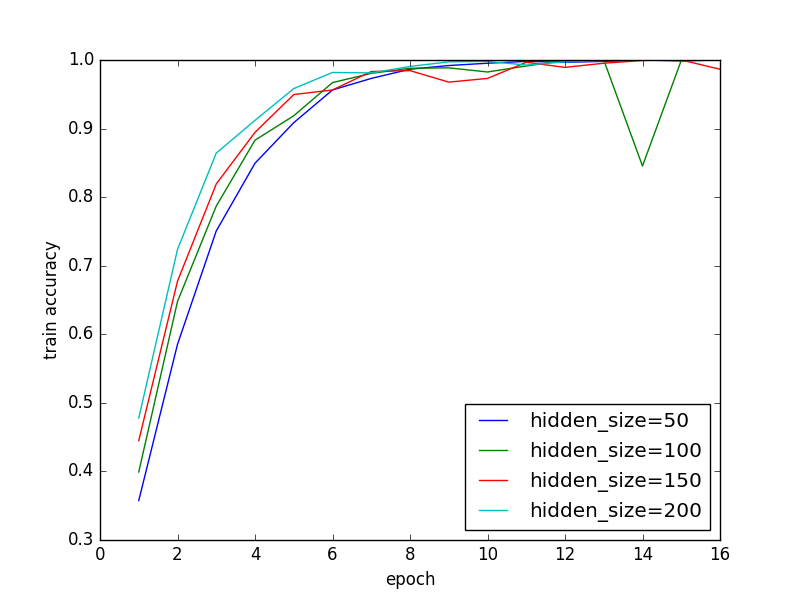
\includegraphics[width=0.7\textwidth]{figures/epoch_train_accu_hs_g.png} 
\caption{Training accuracy vs epoch.}
\end{subfigure}
\begin{subfigure}{0.5\linewidth}
\centering
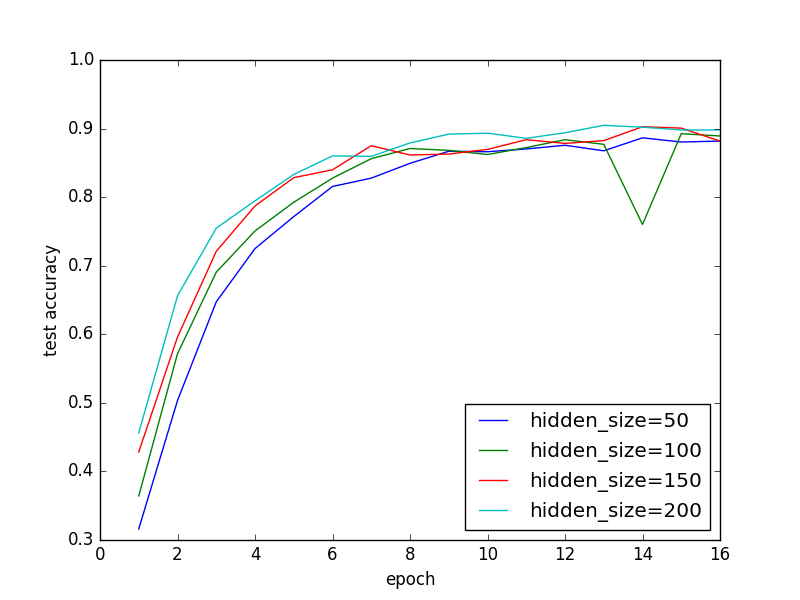
\includegraphics[width=0.7\textwidth]{figures/epoch_test_accu_hs_g.png} 
\caption{Testing accuracy vs epoch.}
\end{subfigure}
\caption{Training and test accuracy for different hidden size on the Gutenberg dataset.}
\label{hs_test_accu_gutenberg_ag}
\end{figure}
%
We then tuned the regularization from 0.00001 to 0.005. The results are shown in Figure \ref{rg_test_accu_c50_ag} and \ref{rg_test_accu_gutenberg_ag}.


\begin{figure}[H]
\begin{subfigure}{0.5\linewidth}
\centering
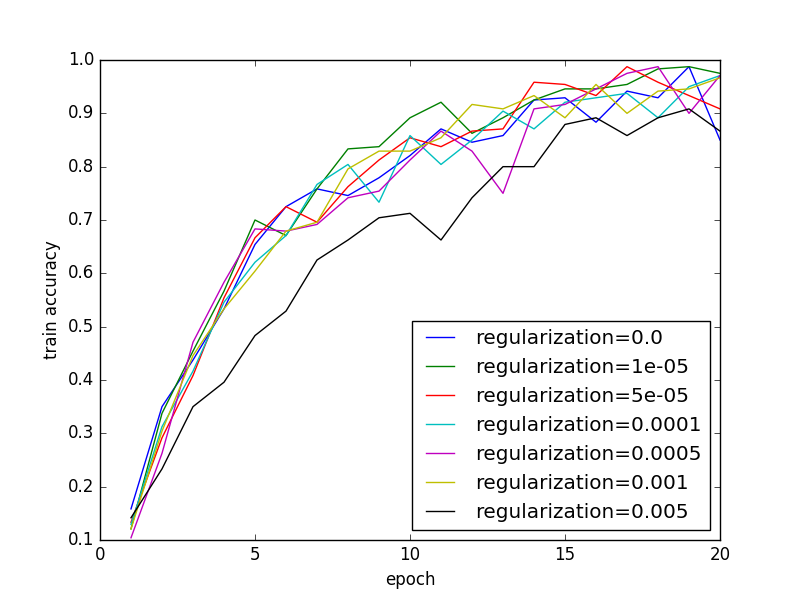
\includegraphics[width=0.7\textwidth]{figures/epoch_train_accu_rg_c.png} 
\caption{Training accuracy vs epoch.}
\end{subfigure}
\begin{subfigure}{0.5\linewidth}
\centering
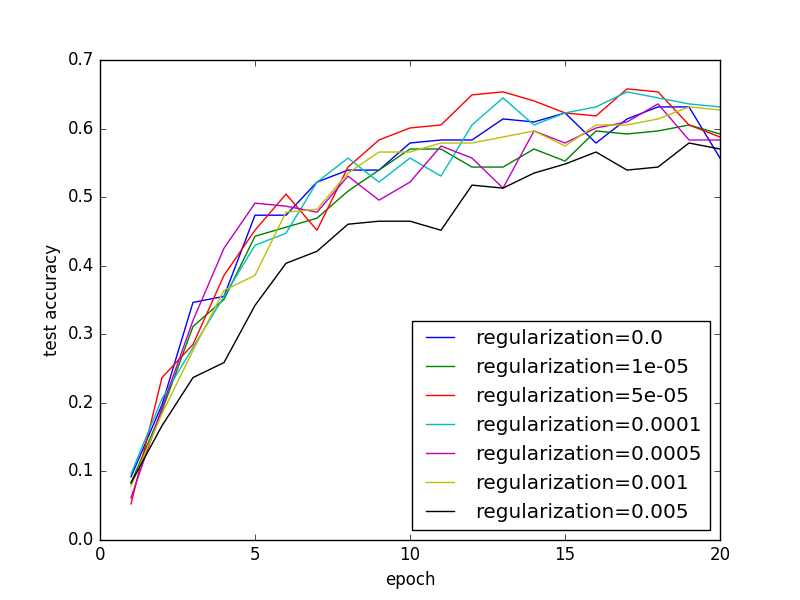
\includegraphics[width=0.7\textwidth]{figures/epoch_test_accu_rg_c.png} 
\caption{Testing accuracy vs epoch.}
\end{subfigure}
\caption{Training and test accuracy for different regularization on the C50 dataset.}
\label{rg_test_accu_c50_ag}
\end{figure}

\begin{figure}[H]
\begin{subfigure}{0.5\linewidth}
\centering
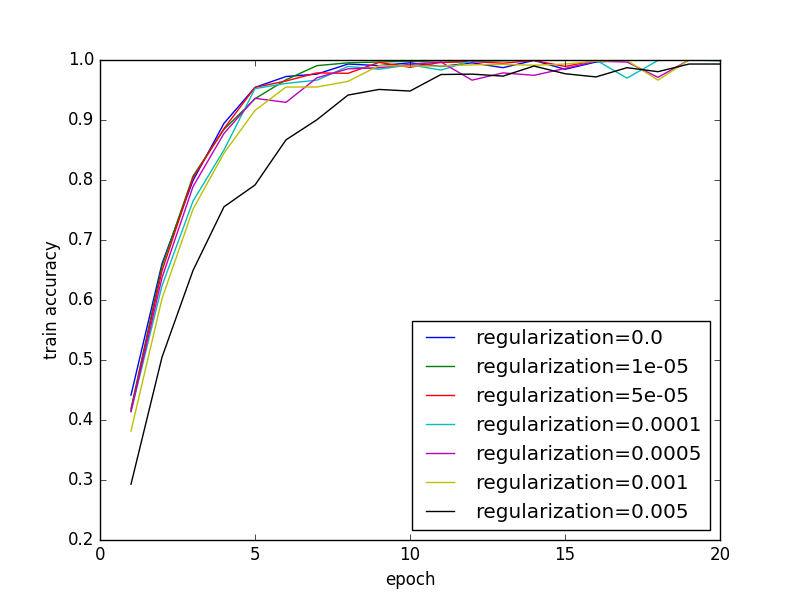
\includegraphics[width=0.7\textwidth]{figures/epoch_train_accu_rg_g.png} 
\caption{Training accuracy vs epoch.}
\end{subfigure}
\begin{subfigure}{0.5\linewidth}
\centering
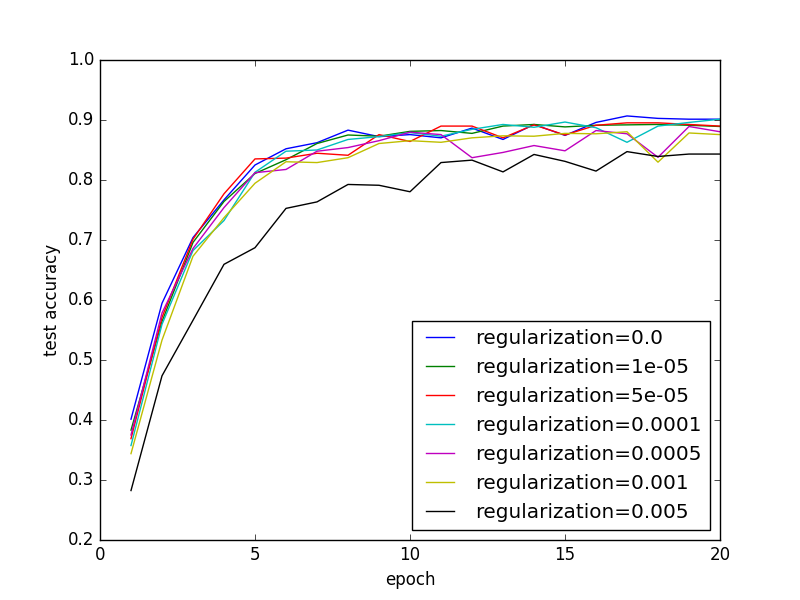
\includegraphics[width=0.7\textwidth]{figures/epoch_test_accu_rg_g.png} 
\caption{Testing accuracy vs epoch.}
\end{subfigure}
\caption{Training and test accuracy for different regularization on the Gutenberg dataset.}
\label{rg_test_accu_gutenberg_ag}
\end{figure}


By comparing the results, we concluded that a hidden size of 150 and a regularization of 0.00005 might be the reasonable choice since they have the highest test accuracy. The confusion matrix for both dataset with the optimized parameter is shown in \ref{fig: confusion_matrix}. The best accuracy for C50 and Gutenberg datasets are 69.1\% and 89.2\% respectively. The F1 score are 0.66 and 0.85 respectively. Also, we concluded that the gutenberg dataset might be too easy. The authors have very distinct wording and styles. This means that it would be less distinctive of the quality of our models. We decided to operate on C50 dataset for other models.

\begin{figure}[H]
\begin{subfigure}{0.5\linewidth}
\centering
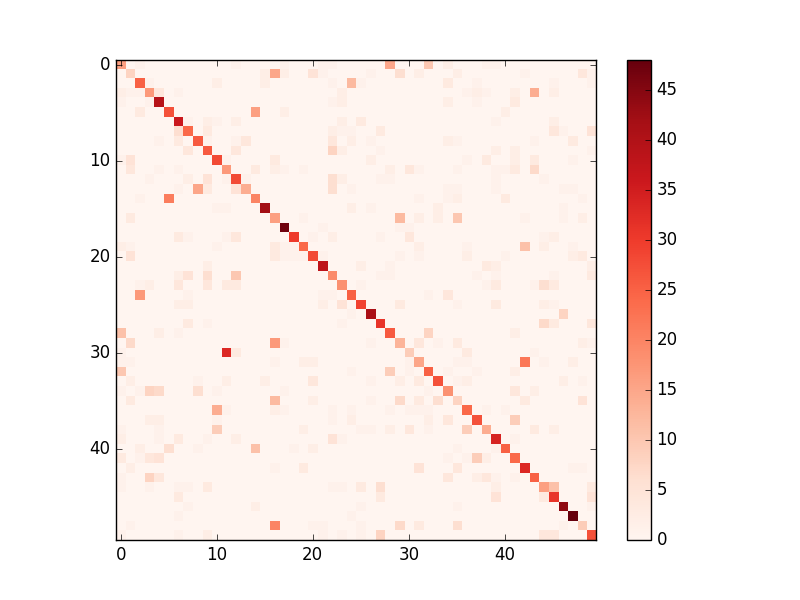
\includegraphics[width=0.8\textwidth]{figures/confusion_matrix_C50_sentence.png} 
\caption{Confusion matrix on C50 dataset. }
\end{subfigure}
\begin{subfigure}{0.5\linewidth}
\centering
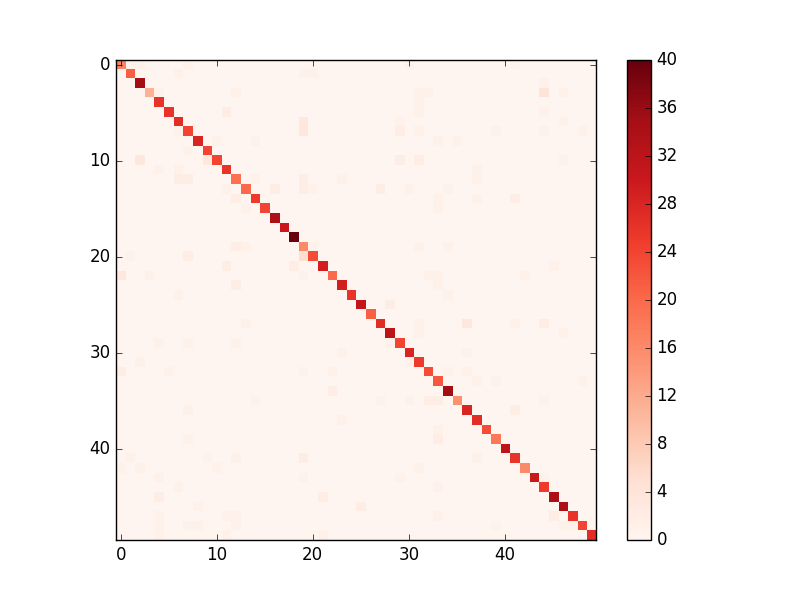
\includegraphics[width=0.8\textwidth]{figures/confusion_matrix_gutenberg_sentence.png} 
\caption{Confusion matrix on Gutenberg dataset.}
\end{subfigure}
\caption{Confusion matrix of the test set on different datasets.}
\label{fig: confusion_matrix}
\end{figure}




\subsection{Article-Level LSTM}
For this model, we also varied the hidden size with C50 dataset and the result is shown in Figure \ref{lstm_hs}. The highest test accuracy of LSTM, however, is 62.7\%, lower than what the previous model can achieve. 
\begin{figure}[H]
\centering
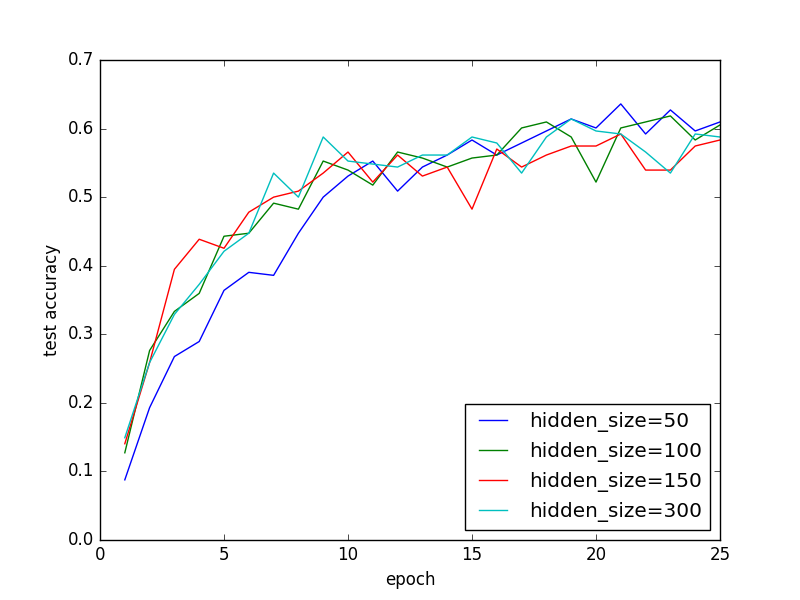
\includegraphics[width=0.4\textwidth]{figures/epoch_test_accu_lstm_c50.png} 
\caption{Test accuracy vs epoch for different hidden size.}
\label{lstm_hs}
\end{figure}

\subsection{Article-Level Siamese Network}

This model relies on a pair-wise dataset that we constructed for C50 dataset. Notice that the ratio between positive and negative samples are 2 : 8, where positive means two input share the same label.

For this model, we varied the parameter $\lambda$, which connects the loss from different parameters. The result on C50 dataset is shown in Table \ref{accu_table}. 

\begin{center}
\begin{tabular}{ |c|c|c|c|c|c| } 
 \hline
 $\lambda$ & 0.0005 &0.001 & 0.005 & 0.01 & 0.5\\
  \hline
 Test accuracy & 97.4\% & 99.8\% & 98.6\% &  97.4\% & 96.3\%  \\ 
 \hline
\end{tabular}
\label{accu_table}
\end{center}

Then we arrived at the optimal $\lambda$ to be 0.001. The train and test accuracy is shown in Figure \ref{siamese_accu}. Note that this evaluation of model has not been done on this dataset before, our test is unique on this dataset. 

\begin{figure}[H]
\centering
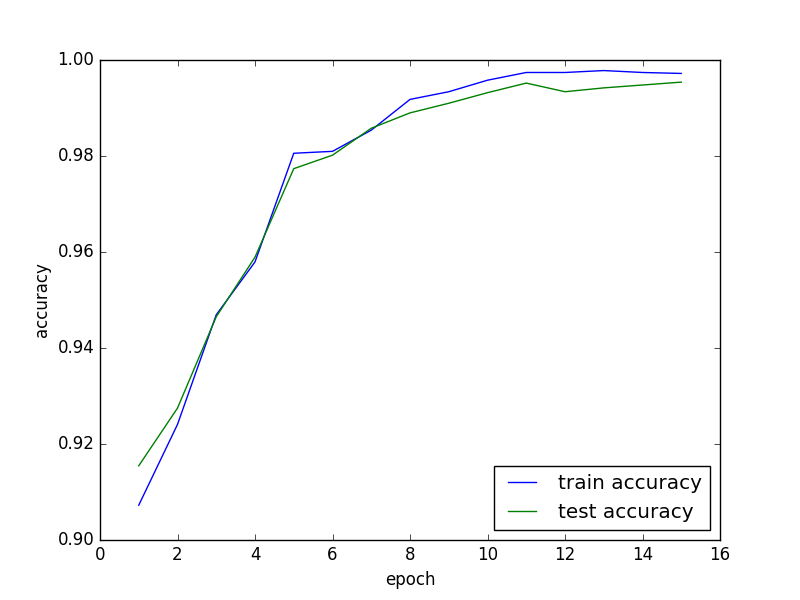
\includegraphics[width=0.4\textwidth]{figures/accu_siamese.png} 
\caption{Training and testing accuracy vs epoch for Siamese network of $\lambda=0.001$.}
\label{siamese_accu}
\end{figure}



\section{Discussion}
\subsection{Limitations}

There are two major limitations in our models. First, in our article-level model, our strategy of representing a sentence is averaging the word vector, which ignores the temporal relationship among words, and also the inside structure of a sentence. Taking these two facts into consideration is promising to improve our model. Second, if one word does not exist in our look-up dictionary, we simply replace that with the magic word. For articles containing a lot of unseen word, the performance of our model loses guarantee.


\subsection{Future Work}
Many future works could be done, such as trying different size of word embeddings, exploiting intra-article attention proposed in \cite{intra}, and methods of representing an article or sentence instead of simply averaging. In addition, other model such as MvRNN or CNN is likely to win over our GRU model on this authorship attribution task, which should be examined. Furthermore, an ensemble of model is promising to give a rise to the accuracy of authorship attribution.

Beyond authorship identification, there are also a great amount of meaningful work worth studying. Recalling our proposed models are capable of extracting style features of a given article, further study might depend on the extracted features to mine more information under the article, e.g., the relationship between two financial reports, or the sentiment change under one person's tweets in a short period.  




\section{Conclusion}

In this project, we studied different deep learning models on authorship identification. we designed and implemented 3 models for authorship identification, and also one model for authorship verification  on C50 dataset and Gutenberg dataset. Article-level GRU performed best on authorship identification, outputing an accuracy of 69.1\% on C50 and 89.2\% on gutenberg dataset. Besides, siamese network achieved an verification accuracy of 99.8\% on both C50 and gutenberg dataset.


\section{Contribution}

For this project, Rao Zhang was responsible for data collecting and preprocessing,  Tianchang He and Chen Qian took responsibility of building and evaluating RNN models. Tianchang He and Rao Zhang did extensive data analysis. Chen Qian designed Siamese Network and put great effort in testing models. 










\newpage
\begin{thebibliography}{99}
\bibitem{pan2014}
Efstathios Stamatatos, Walter Daelemans, Ben Verhoeven, Martin Potthast, Benno Stein, Patrick Juola, Miguel A Sanchez-Perez, and Alberto Barron-Cedeno. Overview of the author identification task at PAN 2014. analysis, 13:31, 2014.
\bibitem{best_known}
M. Koppel, J. Schler, and E. Bonchek-Dokow. Measuring Differentiability: Unmasking Pseudonymous Authors. Journal of Machine Learning Research, 8:1261–1276, 2007.
\bibitem{shortcoming}
C. Sanderson and S.Guenter. Short Text Authorship Attribution via Sequence Kernels, Markov Chains and Author Unmasking: An Investigation. In Proceedings of the International Conference on Empirical Methods in Natural Language Processing, pages 482–491, 2006.
\bibitem{Stamatatos}
Stamatatos E. A survey of modern authorship attribution methods[J]. Journal of the American Society for information Science and Technology, 2009, 60(3): 538-556.
\bibitem{Koppel}
M. Koppel and Y. Winter. Determining if Two Documents are by the Same Author. Journal of the American Society for Information Science and Technology, 65(1):178-187, 2014.
%\bibitem{Efstathios}
%Efstathios Stamatatos, Walter Daelemans, Ben Verhoeven, Martin Potthast, Benno Stein, Patrick Juola, Miguel A Sanchez-Perez, and Alberto Barron-Cede no. Overview of the author-identification task at PAN 2014. analysis, 13:31, 2014.
\bibitem{Rhodes}
Rhodes D. Author attribution with cnns[J]. Avaiable online, 2015.
\bibitem{RCV}
D. D. Lewis, et al. Rcv1: A new benchmark collection for text categorization research[J]. Journal of machine learning research, 2004, 5(Apr): 361-397. 
\bibitem{Reuter} https://archive.ics.uci.edu/ml/datasets/Reuter\_50\_50
\bibitem{Gutenberg} https://www.gutenberg.org/wiki/Main\_Page

\bibitem{glove}
J. Pennington, R. Socher, C. Manning, GloVe: Global Vectors for Word Representation, EMNLP, 2014

\bibitem{garbage}
L. Zhou, H. Wang, News Authorship Identification with Deep Learning, 2016

\bibitem{intra}
Yang, Z., Yang, D., Dyer, C., He, X., Smola, A., \& Hovy, E. (2016). Hierarchical attention networks for document classification. In Proceedings of NAACL-HLT (pp. 1480-1489).

\end{thebibliography}

\end{document}
